\chapter{Magma}

Hệ mật mã Magma được chính phủ Xô Viết chọn làm chuẩn mã hóa.
Cũng giống như hệ mật mã DES, Magma sử dụng mô hình Feistel
cho các vòng mã hóa, được định nghĩa trong GOST 34.12-2015
và còn được đặt tên là GOST 28147-89.

Độ dài khóa là 256 bit. Độ dài khối là 64 bit. Magma biến
đổi trên 32 vòng để cho ra ciphertext.

Magma thực hiện biến đổi trên 32 vòng Feistel. Khối đầu vào 
64 bit được chia thành 2 nửa trái phải, mỗi nửa 32 bit.

\section{Key schedule}

Khóa 256 bit được chia thành 8 cụm khóa con, mỗi khóa con 32 bit.

Nếu ta ký hiệu 256 bit của khóa là $k_{0} k_{1} \ldots k_{254} k_{255}$
thì ta có các khóa con là
\[ \underbrace{k_0 \ldots k_{31}}_{K_0} \underbrace{k_{32} \ldots k_{63}}_{K_1}
    \ldots \underbrace{k_{224} \ldots k_{255}}_{K_7}\]

Từ vòng 1 tới 24 sử dụng lần lượt các khóa $K_0$, $K_1$, ..., $K_7$
rồi lặp lại thứ tự đó.

Từ vòng 24 tới 32 sử dụng theo thứ tự ngược lại, từ $K_7$, $K_6$, ...,
$K_0$.

\begin{figure}[ht]
    \centering
    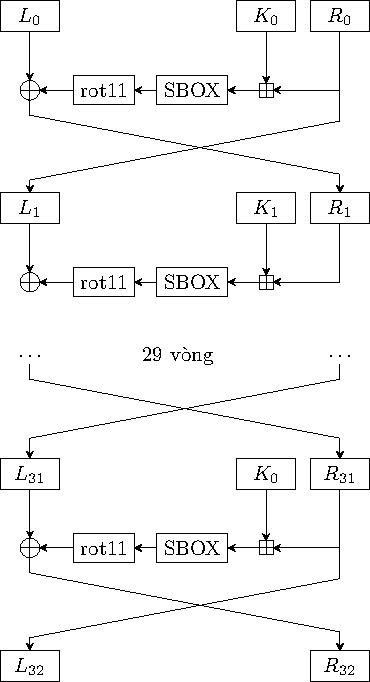
\includegraphics{Magma/blocky.pdf}
    \caption{Mô hình mã khối Magma}
\end{figure}

\section{Round function}

Như ta đã biết, trong mô hình Feistel, mỗi khối plaintext
được chia thành 2 nửa trái phải $(L_0, R_0)$. Sau đó ở mỗi vòng
biến đổi thì

\[L_{i+1} = R_i, \quad, R_{i+1} = L_i \oplus f(R_i, K_i)\]
với $i=0, 1, \ldots$ và $K_i$ là khóa con ở vòng $i$.

Hàm $f$ của Magma khá đơn giản, bao gồm 3 động tác là cộng modulo 
$2^{32}$, SBox và xoay 11 bit.

Đối với việc cộng modulo $2^{32}$, ta xem block $R_i$ và $K_i$ như
những số 32 bit, cộng chúng lại và modulo $2^{32}$. Nghĩa là 
$(R_i + K_i) \bmod 2^{32}$.

Đặt $T_i = (R_i + K_i) \bmod 2^{32}$. Như vậy $T_i$ có 32 bit. Ta 
chia 32 bit này thành 8 cụm 4 bit. Ứng với mỗi cụm 4 bit chúng ta 
cho qua một hoán vị. Như vậy cần 8 hoán vị (SBox). SBox được sử dụng
chung cho tất cả vòng.

Theo wiki thì SBox có thể bí mật. Tuy nhiên việc mã hóa và giải
mã cần sử dụng SBox giống nhau. Do đó thiết bị mã hóa và giải mã
có cùng cơ chế pseudo-random để sinh ra SBox giống nhau.

SBox được quy định theo tiêu chuẩn chính phủ Nga là

\begin{lstlisting}[language=Python]
sbox = [
    [0xC, 0x4, 0x6, 0x2, 0xA, 0x5, 0xB, 0x9, 
        0xE, 0x8, 0xD, 0x7, 0x0, 0x3, 0xF, 0x1],
    [0x6, 0x8, 0x2, 0x3, 0x9, 0xA, 0x5, 0xC, 
        0x1, 0xE, 0x4, 0x7, 0xB, 0xD, 0x0, 0xF],
    [0xB, 0x3, 0x5, 0x8, 0x2, 0xF, 0xA, 0xD, 
        0xE, 0x1, 0x7, 0x4, 0xC, 0x9, 0x6, 0x0],
    [0xC, 0x8, 0x2, 0x1, 0xD, 0x4, 0xF, 0x6, 
        0x7, 0x0, 0xA, 0x5, 0x3, 0xE, 0x9, 0xB],
    [0x7, 0xF, 0x5, 0xA, 0x8, 0x1, 0x6, 0xD, 
        0x0, 0x9, 0x3, 0xE, 0xB, 0x4, 0x2, 0xC],
    [0x5, 0xD, 0xF, 0x6, 0x9, 0x2, 0xC, 0xA, 
        0xB, 0x7, 0x8, 0x1, 0x4, 0x3, 0xE, 0x0],
    [0x8, 0xE, 0x2, 0x5, 0x6, 0x9, 0x1, 0xC, 
        0xF, 0x4, 0xB, 0x0, 0xD, 0xA, 0x3, 0x7],
    [0x1, 0x7, 0xE, 0xD, 0x0, 0x5, 0x8, 0x3, 
        0x4, 0xF, 0xA, 0x6, 0x9, 0xC, 0xB, 0x2],
]
\end{lstlisting}

Nếu $T_i$ được viết dưới dạng 32 bit là $t_{31} t_{30} \ldots t_1 t_0$
thì SBox tương ứng của nó là
\[
    \underbrace{t_{31} \ldots t_{28}}_{S_7}
    \underbrace{t_{27} \ldots t_{24}}_{S_6}
    \ldots
    \underbrace{t_{7} \ldots t_{4}}_{S_1}
    \underbrace{t_3 \ldots t_0}_{S_0}
\]

Nói cách khác, $t_{4i+3} t_{4i+2} t_{4i+1} t_{4i}$ dùng $S_{7-i}$ với
$i = 0, 1, 2, \ldots, 7$.

Cuối cùng, việc xoay trái 11 bit (rot11) chỉ đơn giản là đưa 11 bit đầu
về cuối và đưa 21 bit cuối lên đầu.

Để giải mã ta vẫn sử dụng round function như lúc mã hóa, 
chỉ cần viết với thứ tự ngược lại là được. Như vậy
\[R_i = L_{i+1}, \quad, L_i = R_{i+1} \oplus f(L_{i+1}, K_i)\]
do $R_i = L_{i+1}$. Lưu ý rằng khóa con lúc này là 0 tới 7 cho 
8 vòng đầu, và 7 về 0 (rồi lặp lại) cho 24 vòng sau.